\chapter{VLSI-Systementwurf Praktikum}
	\section{Kurze Beschreibung des Terasic DE0 Board}
	\begin{center}
	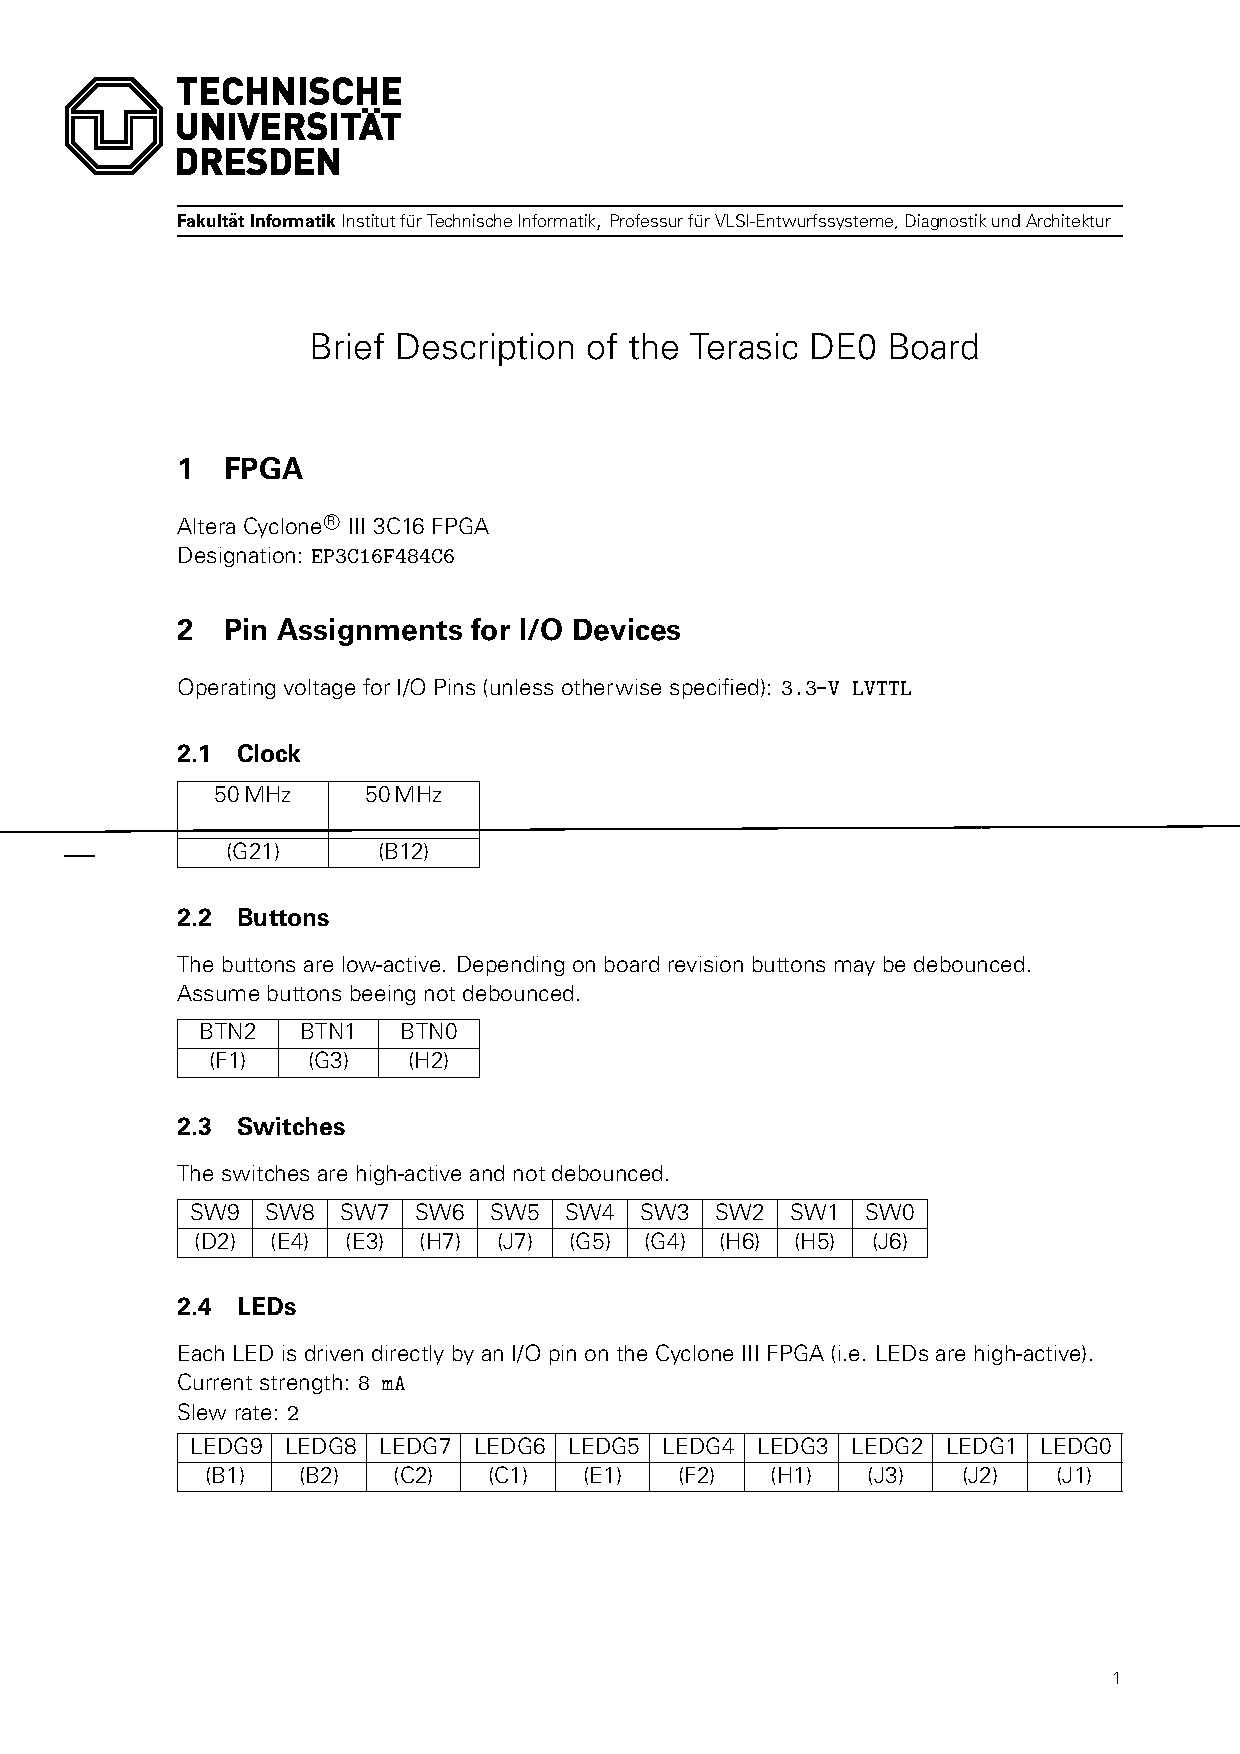
\includegraphics[page=1, width=\linewidth, trim=30mm 30mm 20mm 110mm, clip]{\Path/resources/Praktikum/VLSI/Material/Praktikumsboard/DE0_Description.pdf}
	\begin{center}
	\end{center}
	\includegraphics[page=2, width=\linewidth, trim=30mm 90mm 20mm 30mm, clip]{\Path/resources/Praktikum/VLSI/Material/Praktikumsboard/DE0_Description.pdf}
	\end{center}
	
	\def \Path {/media/Daten/Studium/Skripte/TechnischeInformatik/resources/Praktikum/VLSI/Abgabe/Protokolle}
	\begin{center}
	
\includegraphics[page=1, width=\linewidth, trim=30mm 100mm 20mm 110mm, clip]{\Path/resources/Stoppuhr.pdf}
	\end{center}
	\section{Aufgabe 1 - Binär-Dekoder}
\subsection{Entwurf}
\begin{description}
	\item[Input] 4-Bit Binärzahl durch Schieberegister SW3 ... SW0
	\item[Output] 7-Segmente Darstellung einer Hexadezimalziffer (8 Einzelsignale = 7 Segmente + 1 Punkt)
\end{description}

\begin{tabular}{|c|c|c|c||c|c|c|c|c|c|c|c|c|}
\hline
\multicolumn{4}{|c|}{Input} & \multicolumn{9}{|c|}{Output} \\
\hline
\textsc{SW3} & \textsc{SW2} & \textsc{SW1} & \textsc{SW0} & 
\textsc{Hex} & \textsc{A} & \textsc{B} & \textsc{C} & \textsc{D} & \textsc{E} & \textsc{F} & \textsc{G} & \textsc{dot} \\ 
\hline
\hline
0 & 0 & 0 & 0 & 0 & 0 & 0 & 0 & 0 & 0 & 0 & 1 & 1 \\ 
0 & 0 & 0 & 1 & 1 & 1 & 0 & 0 & 1 & 1 & 1 & 1 & 1 \\
0 & 0 & 1 & 0 & 2 & 0 & 0 & 1 & 0 & 0 & 1 & 0 & 1 \\
0 & 0 & 1 & 1 & 3 & 0 & 0 & 0 & 0 & 1 & 1 & 0 & 1 \\
0 & 1 & 0 & 0 & 4 & 1 & 0 & 0 & 1 & 1 & 0 & 0 & 1 \\
0 & 1 & 0 & 1 & 5 & 0 & 1 & 0 & 0 & 1 & 0 & 0 & 1 \\
0 & 1 & 1 & 0 & 6 & 0 & 1 & 0 & 0 & 0 & 0 & 0 & 1 \\
0 & 1 & 1 & 1 & 7 & 0 & 0 & 0 & 1 & 1 & 1 & 1 & 1 \\
1 & 0 & 0 & 0 & 8 & 0 & 0 & 0 & 0 & 0 & 0 & 0 & 1 \\
1 & 0 & 0 & 1 & 9 & 0 & 0 & 0 & 0 & 1 & 0 & 0 & 1 \\
1 & 0 & 1 & 0 & A & 0 & 0 & 0 & 1 & 0 & 0 & 0 & 1 \\
1 & 0 & 1 & 1 & b & 1 & 1 & 0 & 0 & 0 & 0 & 0 & 1 \\
1 & 1 & 0 & 0 & C & 0 & 1 & 1 & 0 & 0 & 0 & 1 & 1 \\
1 & 1 & 0 & 1 & d & 1 & 0 & 0 & 0 & 0 & 1 & 0 & 1 \\
1 & 1 & 1 & 0 & E & 0 & 1 & 1 & 0 & 0 & 0 & 0 & 1 \\
1 & 1 & 1 & 1 & F & 0 & 1 & 1 & 1 & 0 & 0 & 0 & 1 \\
\hline
\end{tabular}	
\\\\
\ref{lst:01-decoder}~Decoder.vhdl Code
\subsection{Auswertung}
\paragraph{Ressourcenbedarf}
\begin{itemize} 
\item 7 Logik-Elemente
\item 12 Pins 
\end{itemize}

	\begin{center}
	
\includegraphics[page=1, width=\linewidth, trim=30mm 45mm 20mm 198mm, clip]{\Path/resources/Stoppuhr.pdf}
	\end{center}
	\section{Aufgabe 2 - Zeitmessungen}
(nicht Taurus)

\begin{table}[!htb]
\caption{Original, gcc}
\begin{minipage}{.5\linewidth}
\centering
\subsection{Original, gcc, keine flags}
\begin{tabular}{|l|r|r|}
	\hline
	\textsc{Dimension} & \textsc{Runtime} & \textsc{GFLOP/s} \\
	\hline
	\hline
	32  &  0.0002s  & 0.40 \\ 
	\hline 
	64  &  0.0015s  & 0.40 \\ 
	\hline 
	96  &  0.0045s  & 0.40 \\ 
	\hline 
	128  &  0.0115s  & 0.38 \\ 
	\hline 
	160  &  0.0217s  & 0.37 \\ 
	\hline 
	192  &  0.0503s  & 0.36 \\ 
	\hline 
	224  &  0.0651s  & 0.35 \\ 
	\hline 
	256  &  0.1365s  & 0.25 \\ 
	\hline 
	320  &  0.1984s  & 0.33 \\ 
	\hline 
	384  &  0.4676s  & 0.25 \\ 
	\hline 
	448  &  0.5567s  & 0.33 \\ 
	\hline 
	512  &  1.3026s  & 0.21 \\ 
	\hline 
	640  &  2.9606s  & 0.18 \\ 
	\hline 
	768  &  5.5037s  & 0.16 \\ 
	\hline 
	896  & 8.5051s  & 0.17 \\ 
	\hline 
	1024  & 26.0022s  & 0.16 \\ 
	\hline 

\end{tabular}
\end{minipage}%
\begin{minipage}{.5\linewidth}
\centering
\subsection{Original, gcc, -O3}
\begin{tabular}{|l|r|r|}
	\hline
	\textsc{Dimension} & \textsc{Runtime} & \textsc{GFLOP/s} \\
	\hline
	\hline
	32  &  0.0000s  & 1.73 \\ 
	\hline 
	64  &  0.0003s  & 1.85 \\ 
	\hline 
	96  &  0.0009s  & 1.93 \\ 
	\hline 
	128  &  0.0031s  & 1.35 \\ 
	\hline 
	160  &  0.0055s  & 1.56 \\ 
	\hline 
	192  &  0.0104s  & 1.37 \\ 
	\hline 
	224  &  0.0159s  & 1.42 \\ 
	\hline 
	256  &  0.0339s  & 1.00 \\ 
	\hline 
	320  &  0.0537s  & 1.24 \\ 
	\hline 
	384  &  0.1077s  & 1.06 \\ 
	\hline 
	448  &  0.1524s  & 1.18 \\ 
	\hline 
	512  &  0.3500s  & 0.78 \\ 
	\hline 
	640  &  1.6626s  & 0.33 \\ 
	\hline 
	768  &  3.2088s  & 0.29 \\ 
	\hline 
	896  & 5.1806s  & 0.28 \\ 
	\hline 
	1024  & 7.5068s  & 0.29 \\ 
	\hline 

\end{tabular}

\end{minipage}%
\end{table}


\begin{table}[!htb]
\caption{Mit Optimierungen, gcc}
\begin{minipage}{.5\linewidth}
\centering
\subsection{Mit Optimierungen, gcc, keine flags}
\begin{tabular}{|l|r|r|}
	\hline
	\textsc{Dimension} & \textsc{Runtime} & \textsc{GFLOP/s} \\
	\hline
	\hline
	32  &  0.0001s  & 0.61 \\ 
	\hline 
	64  &  0.0009s  & 0.61 \\ 
	\hline 
	96  &  0.0026s  & 0.70 \\ 
	\hline 
	128  &  0.0058s  & 0.71 \\ 
	\hline 
	160  &  0.0115s  & 0.71 \\ 
	\hline 
	192  &  0.0198s  & 0.71 \\ 
	\hline 
	224  &  0.0313s  & 0.72 \\ 
	\hline 
	256  &  0.0465s  & 0.72 \\ 
	\hline 
	320  &  0.0902s  & 0.73 \\ 
	\hline 
	384  &  0.1552s  & 0.73 \\ 
	\hline 
	448  &  0.2451s  & 0.73 \\ 
	\hline 
	512  &  0.3632s  & 0.74 \\ 
	\hline 
	640  &  0.7120s  & 0.74 \\ 
	\hline 
	768  &  1.2261s  & 0.74 \\ 
	\hline 
	896  &  1.9538s  & 0.74 \\ 
	\hline 
	1024  &  2.9417s  & 0.73 \\ 
	\hline 
\end{tabular}
\end{minipage}%
\begin{minipage}{.5\linewidth}
\centering
\subsection{Mit Optimierungen, gcc, -O3}
\begin{tabular}{|l|r|r|}
	\hline
	\textsc{Dimension} & \textsc{Runtime} & \textsc{GFLOP/s} \\
	\hline
	\hline
	32  &  0.0000s  & 2.12 \\ 
	\hline 
	64  &  0.0002s  & 2.24 \\ 
	\hline 
	96  &  0.0006s  & 2.50 \\ 
	\hline 
	128  &  0.0015s  & 2.58 \\ 
	\hline 
	160  &  0.0031s  & 2.56 \\ 
	\hline 
	192  &  0.0052s  & 2.65 \\ 
	\hline 
	224  &  0.0081s  & 2.67 \\ 
	\hline 
	256  &  0.0120s  & 2.75 \\ 
	\hline 
	320  &  0.0239s  & 2.72 \\ 
	\hline 
	384  &  0.0408s  & 2.76 \\ 
	\hline 
	448  &  0.0647s  & 2.77 \\ 
	\hline 
	512  &  0.0941s  & 2.86 \\ 
	\hline 
	640  &  0.1886s  & 2.78 \\ 
	\hline 
	768  &  0.3226s  & 2.81 \\ 
	\hline 
	896  &  0.5146s  & 2.80 \\ 
	\hline 
	1024  &  0.7530s  & 2.85 \\ 
	\hline 
\end{tabular}
\end{minipage}%
\end{table}


\begin{table}[!htb]
\caption{Original, icc}
\begin{minipage}{.5\linewidth}
\centering
\subsection{Original, icc, keine flags}
\begin{tabular}{|l|r|r|}
	\hline
	\textsc{Dimension} & \textsc{Runtime} & \textsc{GFLOP/s} \\
	\hline
	\hline
	32  &  0.0000s  & 1.52 \\ 
	\hline 
	64  &  0.0001s  & 3.67 \\ 
	\hline 
	96  &  0.0003s  & 4.30 \\ 
	\hline 
	128  &  0.0008s  & 4.88 \\ 
	\hline 
	160  &  0.0018s  & 4.87 \\ 
	\hline 
	192  &  0.0030s  & 4.90 \\ 
	\hline 
	224  &  0.0046s  & 4.73 \\ 
	\hline 
	256  &  0.0072s  & 4.73 \\ 
	\hline 
	320  &  0.0125s  & 4.99 \\ 
	\hline 
	384  &  0.0228s  & 5.02 \\ 
	\hline 
	448  &  0.0346s  & 5.17 \\ 
	\hline 
	512  &  0.0533s  & 5.02 \\ 
	\hline 
	640  &  0.1020s  & 5.13 \\ 
	\hline 
	768  &  0.1739s  & 5.15 \\ 
	\hline 
	896  &  0.2743s  & 5.25 \\ 
	\hline 
	1024  &  0.4137s  & 5.19 \\ 
	\hline 
\end{tabular}
\end{minipage}%
\begin{minipage}{.5\linewidth}
\centering
\subsection{Original, icc, -O3}
\begin{tabular}{|l|r|r|}
	\hline
	\textsc{Dimension} & \textsc{Runtime} & \textsc{GFLOP/s} \\
	\hline
	\hline
	32  &  0.0000s  & 1.98 \\ 
	\hline 
	64  &  0.0001s  & 3.69 \\ 
	\hline 
	96  &  0.0004s  & 4.00 \\ 
	\hline 
	128  &  0.0009s  & 4.51 \\ 
	\hline 
	160  &  0.0016s  & 4.67 \\ 
	\hline 
	192  &  0.0031s  & 4.60 \\ 
	\hline 
	224  &  0.0051s  & 4.43 \\ 
	\hline 
	256  &  0.0076s  & 4.40 \\ 
	\hline 
	320  &  0.0144s  & 4.57 \\ 
	\hline 
	384  &  0.0245s  & 4.66 \\ 
	\hline 
	448  &  0.0386s  & 4.67 \\ 
	\hline 
	512  &  0.0582s  & 4.60 \\ 
	\hline 
	640  &  0.1117s  & 4.70 \\ 
	\hline 
	768  &  0.1937s  & 4.69 \\ 
	\hline 
	896  &  0.3035s  & 4.75 \\ 
	\hline 
	1024  &  0.4552s  & 4.73 \\ 
	\hline 
\end{tabular}
\end{minipage}%
\end{table}




\begin{table}[!htb]
\caption{Mit Optimierungen, icc}
\begin{minipage}{.5\linewidth}
\centering
\subsection{Mit Optimierungen, icc, keine flags}
\begin{tabular}{|l|r|r|}
	\hline
	\textsc{Dimension} & \textsc{Runtime} & \textsc{GFLOP/s} \\
	\hline
	\hline
	32  &  0.0000s  & 2.99 \\ 
	\hline 
	64  &  0.0001s  & 5.09 \\ 
	\hline 
	96  &  0.0003s  & 5.41 \\ 
	\hline 
	128  &  0.0007s  & 5.98 \\ 
	\hline 
	160  &  0.0014s  & 5.95 \\ 
	\hline 
	192  &  0.0024s  & 5.65 \\ 
	\hline 
	224  &  0.0041s  & 5.41 \\ 
	\hline 
	256  &  0.0062s  & 5.29 \\ 
	\hline 
	320  &  0.0121s  & 5.45 \\ 
	\hline 
	384  &  0.0202s  & 5.52 \\ 
	\hline 
	448  &  0.0327s  & 5.57 \\ 
	\hline 
	512  &  0.0481s  & 5.61 \\ 
	\hline 
	640  &  0.0928s  & 5.63 \\ 
	\hline 
	768  &  0.1606s  & 5.65 \\ 
	\hline 
	896  &  0.2522s  & 5.70 \\ 
	\hline 
	1024  &  0.3757s  & 5.72 \\ 
	\hline 
\end{tabular}
\end{minipage}%
\begin{minipage}{.5\linewidth}
\centering
\subsection{Mit Optimierungen, icc, -O3}
\begin{tabular}{|l|r|r|}
	\hline
	\textsc{Dimension} & \textsc{Runtime} & \textsc{GFLOP/s} \\
	\hline
	\hline
	32  &  0.0000s  & 2.72 \\ 
	\hline 
	64  &  0.0001s  & 5.07 \\ 
	\hline 
	96  &  0.0003s  & 5.34 \\ 
	\hline 
	128  &  0.0006s  & 5.67 \\ 
	\hline 
	160  &  0.0016s  & 5.60 \\ 
	\hline 
	192  &  0.0024s  & 5.78 \\ 
	\hline 
	224  &  0.0046s  & 5.35 \\ 
	\hline 
	256  &  0.0062s  & 5.32 \\ 
	\hline 
	320  &  0.0122s  & 5.44 \\ 
	\hline 
	384  &  0.0202s  & 5.51 \\ 
	\hline 
	448  &  0.0322s  & 5.58 \\ 
	\hline 
	512  &  0.0482s  & 5.57 \\ 
	\hline 
	640  &  0.0950s  & 5.52 \\ 
	\hline 
	768  &  0.1650s  & 5.50 \\ 
	\hline 
	896  &  0.2561s  & 5.54 \\ 
	\hline 
	1024  &  0.3841s  & 5.58 \\ 
	\hline 
\end{tabular}
\end{minipage}%
\end{table}

	\begin{center}
	
\includegraphics[page=2, width=\linewidth, trim=30mm 130mm 20mm 30mm, clip]{\Path/resources/Stoppuhr.pdf}
	\end{center}
	\section{Aufgabe 3 - Compiler-Flags}

\subsection{-O3}
Bei Verwendung des gcc-Compilers bringt dieser Flag eine Verbesserung der Ausführungszeit vom Faktor 4 mit sich. Allerdings verschlechtert er die Ausführungszeit beim icc.
\subsection{-floop-interchange}
Führt eine Vertauschung von Schleifen aus, ähnlich wie die Code-Optimierung.
\subsection{-funroll-loops}
Nimmt Schleifen auseinander, deren Schritte durch den Compiler vor der Ausführung bestimmt werden können.



	\begin{center}
	
\includegraphics[page=3, width=\linewidth, trim=30mm 100mm 20mm 30mm, clip]{\Path/resources/Stoppuhr.pdf}
	\end{center}
	\section{Aufgabe 4 - Entprell-Automat}
\subsection{Entwurf}
	\paragraph{State-Machine-Charts}\hfill \\

	\paragraph{LED} enthält die Komponente Entprellung und verbindet die Ein- und Ausgangssignale. (\ref{lst:04-led}~LED.vhdl-Code) \\
	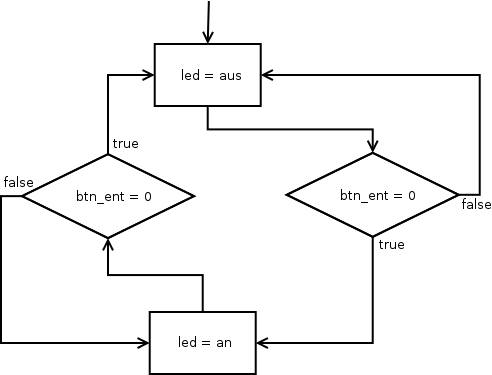
\includegraphics[width=0.7\textwidth]{\Path/resources/04-led.png}
	
	\paragraph{Entprellung} enthält die Komponente Zaehler, der bei der Veränderung des Eingangsignals gestartet wird und für 3ms weitere Änderungen ignoriert. (\ref{lst:04-entprellung}~Entprellung.vhdl-Code) \\
	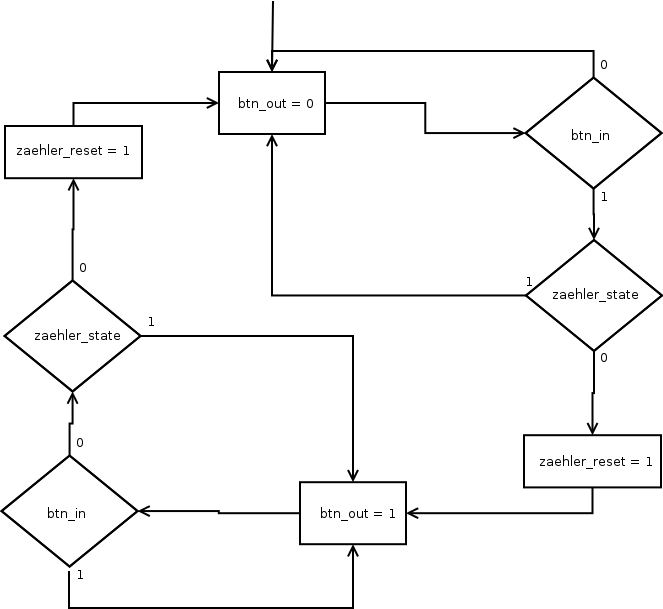
\includegraphics[width=0.8\textwidth]{\Path/resources/04-entpreller.png}


	\paragraph{Zaehler} implementiert einen Zähler, der durch ein Signal definierte Schritte zählt. Ausgegeben wird der aktuelle Zustand des Zählers. Eingegeben ein Reset-Signal. (\ref{lst:04-zaehler}~Zaehler.vhdl-Code) 
	\paragraph{Kopplung} \hfill\\
	Es wird eine synchrone Automatenkopplung über die Ausgangssignale mit einem Taktsignal verwendet.


\subsection{Auswertung}
	\paragraph{Ressourcenbedarf}
	\begin{itemize} 
	\item 86 Logik-Elemente
	\item davon 79 dedizierte Logik-Elemente
	\item 44 Register
	\item 3 Pins 
	\item maximale Taktfrequenz von 178 MHz
	\end{itemize}

	\begin{center}
	
\includegraphics[page=4, width=\linewidth, trim=30mm 130mm 20mm 30mm, clip]{\Path/resources/Stoppuhr.pdf}
	\end{center}
	\section{Aufgabe 5 - HALLO-Anzeige}
\subsection{Entwurf}
	\begin{description}
	\item[zu a)] Es müssen 5 Zeichen kodiert werden (H, A, L, O, Leerzeichen).\\
			\\\(ld\, 5 = 3\)\\\\
			Daher werden für eine Binärkodierung mindestens 3 Bits benötigt.\\\\
			\begin{tabular}{|c|c|c||c|c|c|c|c|c|c|c|c|}
		\hline
		\multicolumn{3}{|c||}{Input} & \multicolumn{9}{|c|}{Output} \\
		\hline
		\textsc{BIT2} & \textsc{BIT1} & \textsc{BIT0} & 
		\textsc{CHAR} & \textsc{A} & \textsc{B} & \textsc{C} & \textsc{D} & \textsc{E} & \textsc{F} & \textsc{G} & \textsc{dot} \\ 
		\hline
		\hline
		0 & 0 & 0 &   & 1 & 1 & 1 & 1 & 1 & 1 & 1 & 1 \\ 
		0 & 0 & 1 & H & 1 & 0 & 0 & 1 & 0 & 0 & 0 & 1 \\
		0 & 1 & 0 & A & 0 & 0 & 0 & 1 & 0 & 0 & 0 & 1 \\
		0 & 1 & 1 & L & 1 & 1 & 1 & 0 & 0 & 0 & 1 & 1 \\
		1 & 0 & 0 & O & 0 & 0 & 0 & 0 & 0 & 0 & 1 & 1 \\
		\hline
	\end{tabular}
	\item[b)] Für das Schieberegister ist der Zählerzustand ein Enable-Signal
	\item[c)]  (\ref{lst:05-hallo}~Hallo.vhdl-Code) 
	\end{description}

	

\subsection{Auswertung}
	\paragraph{Ressourcenbedarf}
	\begin{itemize} 
	\item 73 Logik-Elemente
	\item 61 Register
	\item 34 Pins 
	\item maximale Taktfrequenz von 262 MHz
	\end{itemize}

	\begin{center}
	
\includegraphics[page=4, width=\linewidth, trim=30mm 25mm 20mm 175mm, clip]{\Path/resources/Stoppuhr.pdf}
	
\includegraphics[page=5, width=\linewidth, trim=30mm 200mm 20mm 30mm, clip]{\Path/resources/Stoppuhr.pdf}
	\end{center}
	\section{Aufgabe 6 - Stoppuhr}
\subsection{Entwurf}
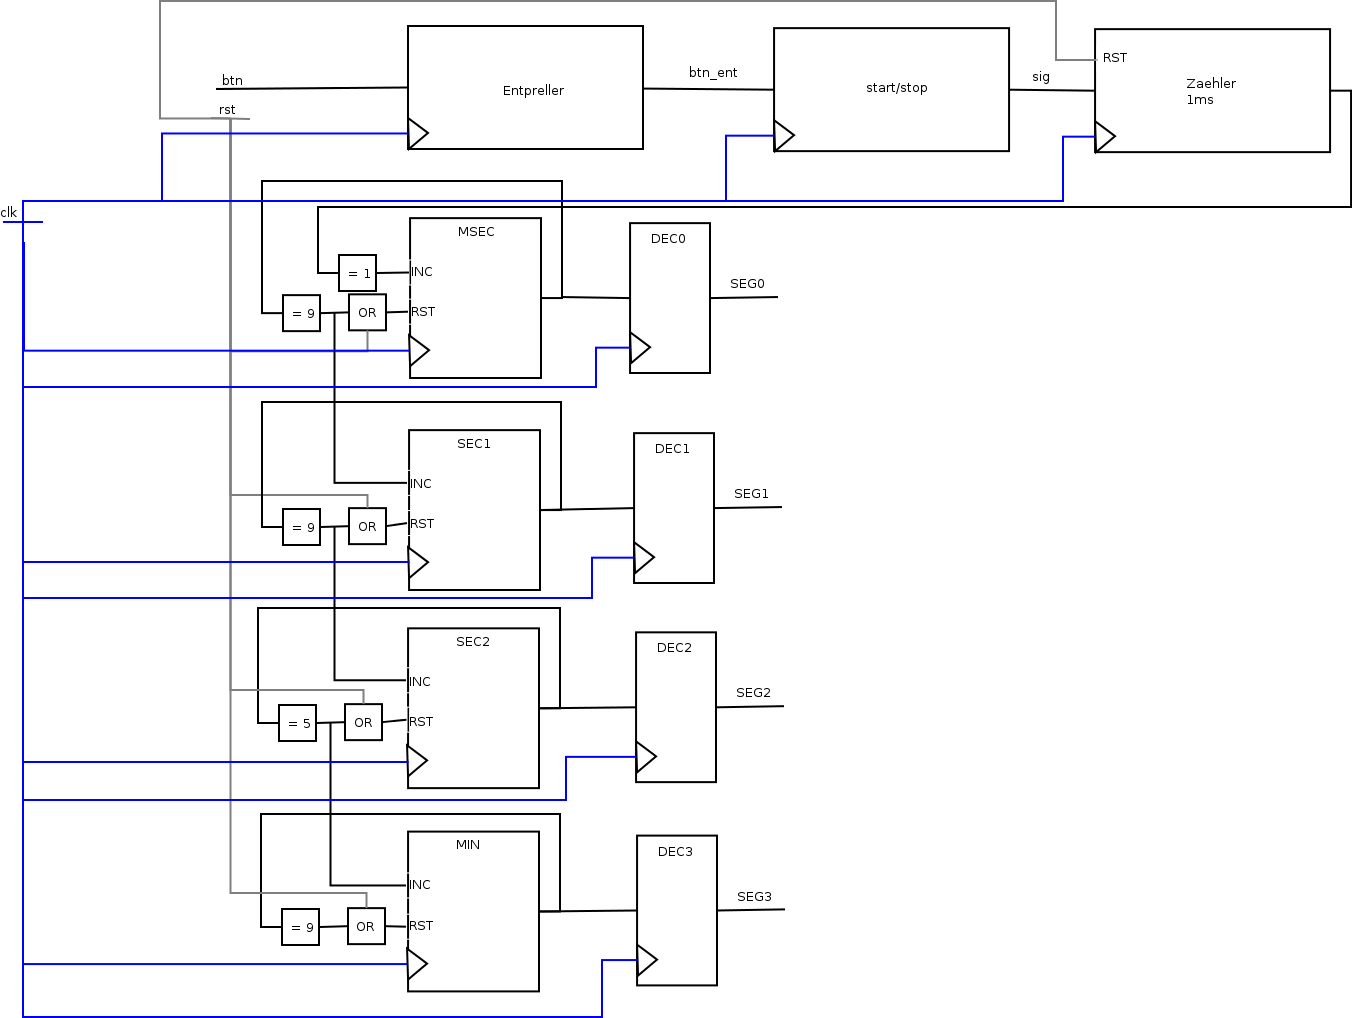
\includegraphics[width=1\textwidth]{\Path/resources/06-stopuhr.png}
	\newpage
	\paragraph{State-Machine-Charts}\hfill \\

		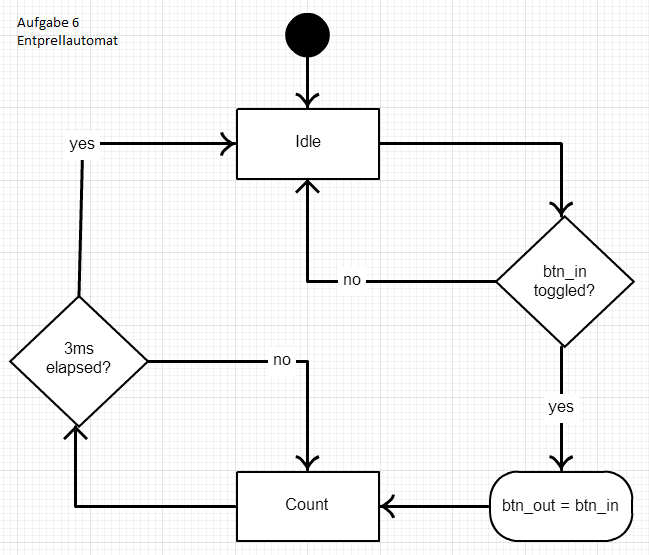
\includegraphics[width=0.8\textwidth]{\Path/resources/06-Entprellautomat.png}
		

		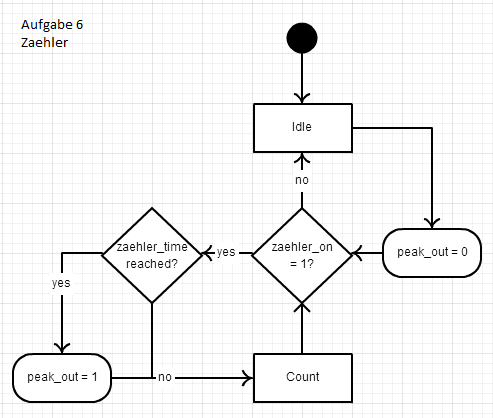
\includegraphics[width=0.7\textwidth]{\Path/resources/06-Zaehler.png}

		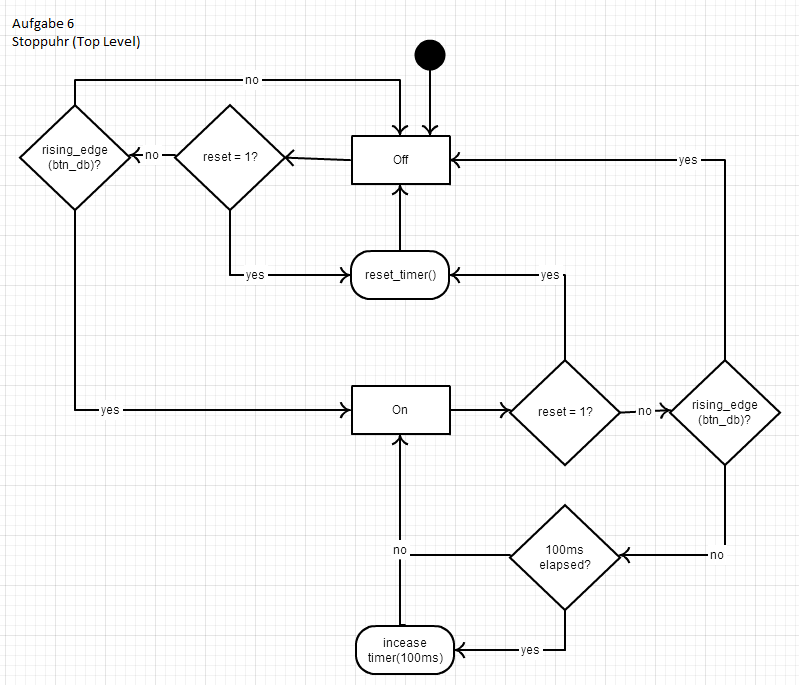
\includegraphics[width=0.7\textwidth]{\Path/resources/06-Stoppuhr.png}
 
	\paragraph{Kopplung} \hfill\\
	Es wird eine synchrone Automatenkopplung über die Ausgangssignale mit einem Taktsignal verwendet.
\subsection{Auswertung}
	\paragraph{Ressourcenbedarf}
	\begin{itemize} 
	\item 163 Logik-Elemente
	\item davon 121 dedizierte Logik-Elemente
	\item 35 Pins 
	\item maximale Taktfrequenz von 225 MHz
	\end{itemize}

	\section{Anhang}
\subsection{Circuit}
\label{lst:circuit}
\lstinputlisting[caption={Circuit.h}, language=C++]{\Path/../Simulator/src/main/Circuit.h}

\subsection{Simulator}
\label{lst:simulator}
\lstinputlisting[caption={Simulator.h}, language=C++]{\Path/../Simulator/src/main/Simulator.h}

\subsection{Solver}
\label{lst:solver}
\lstinputlisting[caption={Solver.h}, language=C++]{\Path/../Simulator/src/main/Solver.h}

\subsection{Parsers}
\label{lst:parsers}
\lstinputlisting[caption={Parsers.h}, language=C++]{\Path/../Simulator/src/parser/Parsers.h}

\subsection{Parser}
\label{lst:parser}
\lstinputlisting[caption={Parser.h}, language=C++]{\Path/../Simulator/src/parser/Parser.h}

\subsection{BENCH}
\label{lst:bench}
\lstinputlisting[caption={BENCH.h}, language=C++]{\Path/../Simulator/src/parser/BENCH.h}

\subsection{Gates}
\label{lst:gates}
\lstinputlisting[caption={Gates.h}, language=C++]{\Path/../Simulator/src/gates/Gates.h}

\subsection{Gate}
\label{lst:gate}
\lstinputlisting[caption={Gate.h}, language=C++]{\Path/../Simulator/src/gates/Gate.h}

\subsection{Input}
\label{lst:input}
\lstinputlisting[caption={Input.h}, language=C++]{\Path/../Simulator/src/gates/Input.h}

\subsection{DFF}
\label{lst:dff}
\lstinputlisting[caption={DFF.h}, language=C++]{\Path/../Simulator/src/gates/DFF.h}

\subsection{Output}
\label{lst:output}
\lstinputlisting[caption={Output.h}, language=C++]{\Path/../Simulator/src/gates/Output.h}
\newpage


	\def \Path {/media/Daten/Studium/Skripte/TechnischeInformatik}


\chapter{Entwurf eingebetteter Systeme: Schaltkreisvalidation}
	
	\def \Path {/media/Daten/Studium/Skripte/TechnischeInformatik/resources/Praktikum/Mikrorechner/Protokolle}
	\section{Programm}

\subsection{Entwurf}
\subsubsection{Circuit}
Das Grundgerüst des Programms bildet die \code{Circuit}-Klasse, die einen Schaltkreis und seine Funktionalitäten implementiert. Die Eingangsbelegung des Schaltkreises wird durch eine Zustandsvariable \code{unsigned int state} repräsentiert, die einen Wert zwischen 0 und $2^N$ annehmen kann, wobei $N$ die Anzahl der Eingänge ist. 
\\\\
Die Eingänge (\code{Input}-Objekte), Gatter (\code{Gate}-Objekte) und Ausgänge (\code{Output}-Objekte) werden in jeweils eigenen Maps abgelegt, deren Keys vom Typ \code{std::string} die Bezeichner der jeweiligen Objekte sind. Alle Gatter sind als Klassen implementiert, die von der abstrakten Klasse \code{Gate} erben. Bei manchen Gattern - wie AND, Or, usw. - können beliebig viele Eingänge definiert werden. Ein Gattereingang ist ein Zeiger, auf entweder den Wert eines \code{Input}-Objektes oder auf den Ausgang eines anderen \code{Gate}-Objektes. Die Ein- und Ausgänge der Gatter sind vom Typ \code{bool}.
\\\\
Bei der Simulation eines Schaltkreises wird über den \code{state} der \code{Circuit}-Klasse iteriert und dessen Wert in Binärdarstellung auf die Eingänge abgebildet. Nach jeder neuen Eingangsbelegung müssen die Gatter durchlaufen werden, bis das neue Signal die Ausgänge erreicht.

\subsubsection{Parser}
Zum Parsen wird die Klasse \code{Parser} als Grundgerüst zur Verfügung gestellt, wobei die genauere Implementierung für unterschiedliche Benchmarks in von dieser Klasse erbenden Klassen verschoben wurde. Für das Benchmark BENCH ist eine solche gleichnamige Klasse vorhanden. 
\\\\
Ein Parser kann Schaltkreise aus Dateien lesen und diese anschliesend als \code{Circuit}-Objekte zurückgeben.
\\\\
Der Parser für das BENCH-Format geht davon aus, dass in der einzulesenden Datei zuerst alle Eingänge (INPUT), dann die Ausgänge (OUTPUT), danach die ggf. vorhandenen FlipFlops (DFF) und zuletzt die restlichen Gatter definiert werden. 
\\\\
Um einen Schaltkreis aus einer Datei zu Parsen, müssen dem Programm die Argumente \\\code{-p BENCHMARK DATEI} mitgeteilt werden.

\subsubsection{Simulator}
Die Klasse \code{Simulator} enthält eine Liste von geparsten \code{Circuit}-Objekten, die simuliert werden können. Dazu wird wieder über den Zustand der Schaltkreise iteriert.
\\\\
Um zum Beispiel zwei Schaltkreise aus Dateien zu parsen und zu Simulieren müssen folgende Argumente übergeben werden:\\
\code{-p BENCHMARK1 DATEI1 -p BENCHMARK2 DATEI2 -s}

	
	\newpage
	\subsection{Äquivalenzprüfung duch Simulation}

\subsubsection{Voraussetzungen}
\begin{itemize}
	\item Schaltkreise müssen gleichviele Eingänge bzw. Ausgänge besitzen
	\item falls in einem Schaltkreis ein Eingang bzw. Ausgang vorkommt, muss ein gleichnamiger Eingang bzw. Ausgang auch in den anderen Schaltkreisen vorkommen
	\item es können beliebig viele Schaltkreise verglichen werden, falls einer nicht äquivalent mit einem anderen ist, wird \code{false} zurückgegeben
	\item ist kein Schaltkreis definiert, wird \code{false} zurückgegeben
	\item ist nur ein Schaltkreis definiert, wird \code{true} zurückgegeben

\end{itemize}

\subsubsection{Vorgehen}
\begin{enumerate}
	\item über mögliche Zustände ($2^N$ mit N ... Anzahl der Eingänge) iterieren

	\begin{enumerate}
		\item durch Schaltkreise iterieren
		\begin{enumerate}
			\item Zustand auf Eingänge abbilden
			\item Schaltkreis traversieren und Ausgangsbelegung ermitteln
		\end{enumerate}
		\item Belegungen mit denen des vorangegangenen Schaltkreises Vergleichen
		\item Bei unterschiedlicher Belegung wird \code{false} zurückgegeben
		\item Sonst wird die Iteration über die Zustände fortgesetzt
	\end{enumerate}
	
	\item wurde über alle $2^N$ Zustände iteriert und keine Varianz der Ausgangsbelegung bei den Schaltkreisen festgestellt, wird \code{true} zurückgegeben
\end{enumerate}


\subsubsection{Implementierung}
Für alle Circuits werden die möglichen Inputs berechnet und die erhaltenen Outputs miteinander verglichen. Sollte dabei ein Circuit enthalten sein, der abweicht, wird false zurückgegeben (Circuits sind nicht äquivalent). 

	
	\newpage
	\subsection{Äquivalenzprüfung durch SAT-Solver}

\subsubsection{Voraussetzungen}
\begin{itemize}
	\item Schaltkreise müssen gleichviele Eingänge bzw. Ausgänge besitzen
	\item falls in einem Schaltkreis ein Eingang bzw. Ausgang vorkommt, muss ein gleichnamiger Eingang bzw. Ausgang auch in den anderen Schaltkreisen vorkommen
	\item es können beliebig viele Schaltkreise verglichen werden, falls einer nicht äquivalent mit einem anderen ist, wird \code{false} zurückgegeben
	\item ist kein Schaltkreis definiert, wird \code{false} zurückgegeben
	\item ist nur ein Schaltkreis definiert, wird \code{true} zurückgegeben

\end{itemize}


\subsubsection{Vorgehen}
\begin{enumerate}
	\item es wird über alle Schaltkreise iteriert
	
	\begin{enumerate}
		\item die KNFs aller Gatter werden ermittelt
		\item falls der Schaltkreis nicht der erste ist, werden seine Eingänge mit denen des ersten Schaltkreises verbunden d.h. die Identität wird duch eine KNF dargestellt
		\item falls der Schaltkreis nicht der erste ist, werden seine Ausgänge XOR mit denen des ersten Schaltkreises verbunden d.h. als KNF dargestellt
	\end{enumerate}
	
	\item alle Ausgänge der XOR-Verbindungen werden OR verküpft, d.h. es wird eine Klausel gebildet, die alle diese Ausgänge enthält
	\subitem lässt sich eine dieser Variablen auf \code{true} abbilden (die These ist SATISFIABLE), dann sind die definierten Schaltkreise nicht äquivalent 
	\item gesamte KNF wird in Datei geschrieben und der SATsolver gestartet
\end{enumerate}


\subsubsection{Implementierung}
Der verwendete SAT-Solver ist miniSAT in der Version 1.14 als Binary. Die generierten KNF-Klauseln werden in eine Datei mit dem Namen cnf geschrieben und anschliesend vom SAT-Solver gelesen. Die jeweiligen Gatter-Klassen sind so implementiert, dass sie ihre Funktion als KNF darstellen können. Die Klasse \code{Solver} enthält einen Zähler für die Benennung der KNF-Variablen.

	
	\newpage
	\chapter{Versuche}

\section{1. Versuch}

\begin{tabular}{|l|c|c|}
	\hline
	\textsc{Benchmarks} & tests/01-test/s344.bench & tests/01-test/s349.bench \\
	\hline
	\hline
	\textsc{Parser} & BENCH & BENCH \\
	\hline
	\textsc{Inputs} & 9 & 9 \\
	\hline
	\textsc{DFFs} & 15 & 15 \\
	\hline
	\textsc{Outputs} & 11 & 11 \\
	\hline
	\textsc{Gatter} & 160 & 161 \\		
	\hline
	\textsc{Zeit in Sekunden} & 0.105102 &  0.103989 \\ 
	\hline
	\hline
	\textsc{Äquivalenzcheck durch SAT-Solving} & \multicolumn{2}{|c|}{äquivalent} \\
	\hline
	\textsc{Zeit in Sekunden} & \multicolumn{2}{|c|}{0.196012} \\
	\hline
	\hline
	\textsc{Äquivalenzcheck durch Simmulierung} & \multicolumn{2}{|c|}{nicht ausgeführt} \\
	\hline
	\textsc{Zeit in Sekunden} & \multicolumn{2}{|c|}{ewig} \\
	\hline
\end{tabular}
\\\\ 
Zu lange Ausführungszeiten für den Simulator.

\section{2. Versuch}

\begin{tabular}{|l|c|c|}
	\hline
	\textsc{Benchmarks} & tests/02-test/s298.bench & tests/02-test/s298.bench \\
	\hline
	\hline
	\textsc{Parser} & BENCH & BENCH \\
	\hline
	\textsc{Inputs} & 3 & 3 \\
	\hline
	\textsc{DFFs} & 14 & 14 \\
	\hline
	\textsc{Outputs} & 6 & 6 \\
	\hline
	\textsc{Gatter} & 119 & 119 \\		
	\hline
	\textsc{Zeit in Sekunden} & 0.079251 &  0.05012 \\ 
	\hline
	\hline
	\textsc{Äquivalenzcheck durch SAT-Solving} & \multicolumn{2}{|c|}{äquivalent} \\
	\hline
	\textsc{Zeit in Sekunden} & \multicolumn{2}{|c|}{0.096006} \\
	\hline
	\hline
	\textsc{Äquivalenzcheck durch Simmulierung} & \multicolumn{2}{|c|}{äquivalent} \\
	\hline
	\textsc{Zeit in Sekunden} & \multicolumn{2}{|c|}{2034.31} \\
	\hline
\end{tabular}

\section{3. Versuch}

\begin{tabular}{|l|c|c|}
	\hline
	\textsc{Benchmarks} & tests/03-test/s298.bench & tests/03-test/s298a.bench \\
	\hline
	\hline
	\textsc{Parser} & BENCH & BENCH \\
	\hline
	\textsc{Inputs} & 3 & 3 \\
	\hline
	\textsc{DFFs} & 14 & 14 \\
	\hline
	\textsc{Outputs} & 6 & 6 \\
	\hline
	\textsc{Gatter} & 119 & 119 \\		
	\hline
	\textsc{Zeit in Sekunden} & 0.048399 &  0.047988 \\ 
	\hline
	\hline
	\textsc{Äquivalenzcheck durch SAT-Solving} & \multicolumn{2}{|c|}{nicht äquivalent} \\
	\hline
	\textsc{Zeit in Sekunden} & \multicolumn{2}{|c|}{0.100006} \\
	\hline
	\hline
	\textsc{Äquivalenzcheck durch Simmulierung} & \multicolumn{2}{|c|}{nicht äquivalent} \\
	\hline
	\textsc{Zeit in Sekunden} & \multicolumn{2}{|c|}{0.016245} \\
	\hline
\end{tabular}

\section{4. Versuch}

\begin{tabular}{|l|c|c|}
	\hline
	\textsc{Benchmarks} & tests/04-test/c17.bench & tests/04-test/c17a.bench \\
	\hline
	\hline
	\textsc{Parser} & BENCH & BENCH \\
	\hline
	\textsc{Inputs} & 5 & 5 \\
	\hline
	\textsc{DFFs} & 0 & 0 \\
	\hline
	\textsc{Outputs} & 2 & 2 \\
	\hline
	\textsc{Gatter} & 6 & 6 \\		
	\hline
	\textsc{Zeit in Sekunden} & 0.002447 & 0.00174 \\ 
	\hline
	\hline
	\textsc{Äquivalenzcheck durch SAT-Solving} & \multicolumn{2}{|c|}{nicht äquivalent} \\
	\hline
	\textsc{Zeit in Sekunden} & \multicolumn{2}{|c|}{0.004} \\
	\hline
	\hline
	\textsc{Äquivalenzcheck durch Simmulierung} & \multicolumn{2}{|c|}{nicht äquivalent} \\
	\hline
	\textsc{Zeit in Sekunden} & \multicolumn{2}{|c|}{0.000122} \\
	\hline
\end{tabular}

\section{5. Versuch}

\begin{tabular}{|l|c|c|}
	\hline
	\textsc{Benchmarks} & tests/05-test/c17.bench & tests/05-test/c17a.bench \\
	\hline
	\hline
	\textsc{Parser} & BENCH & BENCH \\
	\hline
	\textsc{Inputs} & 5 & 5 \\
	\hline
	\textsc{DFFs} & 0 & 0 \\
	\hline
	\textsc{Outputs} & 2 & 2 \\
	\hline
	\textsc{Gatter} & 6 & 7 \\		
	\hline
	\textsc{Zeit in Sekunden} & 0.002533 & 0.001905 \\ 
	\hline
	\hline
	\textsc{Äquivalenzcheck durch SAT-Solving} & \multicolumn{2}{|c|}{äquivalent} \\
	\hline
	\textsc{Zeit in Sekunden} & \multicolumn{2}{|c|}{0} \\
	\hline
	\hline
	\textsc{Äquivalenzcheck durch Simmulierung} & \multicolumn{2}{|c|}{äquivalent} \\
	\hline
	\textsc{Zeit in Sekunden} & \multicolumn{2}{|c|}{ 0.001855} \\
	\hline
\end{tabular} \\\\
Veränderung: ein NAND-Gatter durch ein AND und ein NOT ersetzt. Ergebnis korrekt.


\section{6. Versuch}

\begin{tabular}{|l|c|c|}
	\hline
	\textsc{Benchmarks} & tests/06-test/c6288.bench & tests/05-test/c6288a.bench \\
	\hline
	\hline
	\textsc{Parser} & BENCH & BENCH \\
	\hline
	\textsc{Inputs} & 32 & 32 \\
	\hline
	\textsc{DFFs} & 0 & 0 \\
	\hline
	\textsc{Outputs} & 32 & 32 \\
	\hline
	\textsc{Gatter} & 2416 & 2416 \\		
	\hline
	\textsc{Zeit in Sekunden} & 8.64887 & 8.4408 \\ 
	\hline
	\hline
	\textsc{Äquivalenzcheck durch SAT-Solving} & \multicolumn{2}{|c|}{nicht äquivalent} \\
	\hline
	\textsc{Zeit in Sekunden} & \multicolumn{2}{|c|}{17.3411} \\
	\hline
	\hline
	\textsc{Äquivalenzcheck durch Simmulierung} & \multicolumn{2}{|c|}{nicht äquivalent} \\
	\hline
	\textsc{Zeit in Sekunden} & \multicolumn{2}{|c|}{6.16808} \\
	\hline
\end{tabular} \\\\
Veränderung: 2 Gatter geändert. 

	
	\newpage
	\section{Anhang}
\subsection{Circuit}
\label{lst:circuit}
\lstinputlisting[caption={Circuit.h}, language=C++]{\Path/../Simulator/src/main/Circuit.h}

\subsection{Simulator}
\label{lst:simulator}
\lstinputlisting[caption={Simulator.h}, language=C++]{\Path/../Simulator/src/main/Simulator.h}

\subsection{Solver}
\label{lst:solver}
\lstinputlisting[caption={Solver.h}, language=C++]{\Path/../Simulator/src/main/Solver.h}

\subsection{Parsers}
\label{lst:parsers}
\lstinputlisting[caption={Parsers.h}, language=C++]{\Path/../Simulator/src/parser/Parsers.h}

\subsection{Parser}
\label{lst:parser}
\lstinputlisting[caption={Parser.h}, language=C++]{\Path/../Simulator/src/parser/Parser.h}

\subsection{BENCH}
\label{lst:bench}
\lstinputlisting[caption={BENCH.h}, language=C++]{\Path/../Simulator/src/parser/BENCH.h}

\subsection{Gates}
\label{lst:gates}
\lstinputlisting[caption={Gates.h}, language=C++]{\Path/../Simulator/src/gates/Gates.h}

\subsection{Gate}
\label{lst:gate}
\lstinputlisting[caption={Gate.h}, language=C++]{\Path/../Simulator/src/gates/Gate.h}

\subsection{Input}
\label{lst:input}
\lstinputlisting[caption={Input.h}, language=C++]{\Path/../Simulator/src/gates/Input.h}

\subsection{DFF}
\label{lst:dff}
\lstinputlisting[caption={DFF.h}, language=C++]{\Path/../Simulator/src/gates/DFF.h}

\subsection{Output}
\label{lst:output}
\lstinputlisting[caption={Output.h}, language=C++]{\Path/../Simulator/src/gates/Output.h}
\newpage


	\def \Path {/media/Daten/Studium/Skripte/TechnischeInformatik}
